\documentclass[10pt]{article}
\usepackage{amsmath}
\usepackage{amssymb}
\usepackage{amsthm}
\usepackage{cases}

\usepackage{graphicx}
\usepackage{float}

\title{Projet automatique}
\author{David Castro et Anatole Hernot}
\date{16 décembre 2021}

\begin{document}
\maketitle
\theoremstyle{definition}

\section{Système en boucle ouverte}

\subsection*{Équation d'état}

État $X = (x, v = \dot x, \theta, q = \dot{\theta})$, $u$, l'entrée de commande, $d$, l'entrée de perturbation, $x_m$ et $\theta_m$ les mesures et $x_m$ la sortie à commander.

\vspace{10px}

\noindent On a alors :  $\dot X = \begin{bmatrix} \dot x \\ \dot v \\ \dot \theta \\ \dot q \end{bmatrix} =
\begin{bmatrix} v \\ x q^2 + g \sin \theta \\ q \\ \frac{gx \cos \theta + u + d - 2xqv}{\alpha + x^2} \end{bmatrix}$
avec $\alpha = \frac{J}{m}$.

\subsection*{Point d'équilibre}

\[ \begin{cases} \bar v = 0 \\ \bar x \bar q^2 + g \sin \bar{\theta}  = 0 \\ \bar q = 0 \\ \frac{g \bar x \cos \bar{\theta} + \bar u + \bar d - 2 \bar x \bar q \bar v}{\alpha + \bar x^2} = 0 \end{cases} \]

\[ \begin{cases} \bar v = 0 \\ \sin \bar{\theta}  = 0 \\ \bar q = 0 \\ g \bar x \cos \bar{\theta} + \bar u + \bar d = 0 \end{cases} \]

\vspace{10px}

\noindent Il y a donc deux points d'équilibre : $\left( - \frac{\bar u + \bar d}{g}, 0, 0, 0 \right)$ et $\left( \frac{\bar u + \bar d}{g}, 0, \pi, 0 \right)$.

\subsection*{Linéarisation}

On linéarise au premier point d'équilibre car si on atteint $\theta = \pi$, cela signifie que le rail s'est retourné et donc que la bille est tombée.

\vspace{10px}

\noindent Le système linéarisé tangent en ce point est :

\begin{align}
\delta \dot X &=
	\begin{bmatrix} 
		\delta v \\
		2 \bar x \bar q \delta q + g \delta \theta \\
		\delta q \\
		\frac{g \delta x + \delta u + \delta d - 2 \bar q \bar v \delta x}{\alpha + \bar x^2} - 2 \bar x \delta x \frac{g \bar x + \bar u + \bar d}{\left( \alpha + \bar x^2 \right)^2}
	\end{bmatrix} \notag \\
	&= \begin{bmatrix} 
		\delta v \\
		g \delta \theta \\
		\delta q \\
		\frac{g \delta x + \delta u + \delta d}{\left( \alpha + \bar x^2 \right)^2}
	\end{bmatrix} \notag \\
	&= \underbrace{
	\begin{bmatrix}
		0 & 1 & 0 & 0 \\
		0 & 0 & g & 0 \\
		0 & 0 & 0 & 1 \\
		\frac{g}{\alpha + \bar x^2} & 0 & 0 & 0
	\end{bmatrix}
	}_{A}
	\delta X
	+
	\underbrace{
	\begin{bmatrix}
		0 & 0 \\
		0 & 0 \\
		0 & 0 \\
		\frac{g}{\alpha + \bar x^2} & \frac{g}{\alpha + \bar x^2}
	\end{bmatrix}
	}_{B}
	\delta e \notag
\end{align}

\subsection*{Calcul des valeurs propres}

\begin{align}
	\chi_A (X) &=
	\begin{vmatrix}
		X & -1 & 0 & 0 \\
		0 & X & -g & 0 \\
		0 & 0 & X & -1 \\
		- \frac{g}{\alpha + \bar x^2} & 0 & 0 & X
	\end{vmatrix} \notag \\
	&= X \begin{vmatrix}
		X & -g & 0 \\
		0 & X & -1 \\
		0 & 0 & X
	\end{vmatrix} + 
	\frac{g}{\alpha + \bar x^2} \begin{vmatrix}
		-1 & 0 & 0 \\
		X & -g & 0 \\
		0 & X & -1
	\end{vmatrix} \notag \\
	&= X^4 - \frac{g^2}{\alpha + \bar x^2} \notag
\end{align}

\noindent D'où $\mathrm{Sp} \left( A \right) = \{ \beta ; - \beta ; \beta i ; - \beta i\}$ avec
$\beta =  \sqrt[4]{\frac{g^2}{\alpha + \bar x^2}}  > 0$. Donc le système linéarisé est ue-instable.

\section{Étude préliminaire en boucle fermée}

\subsection*{Ajout d'un contrôleur sur $x$}

Pour tâcher de rendre le système stable au point d'équilibre, on pose un contrôleur proportionnel-dérivé
au niveau de la position :

\[
	\delta u = - k ( \delta x_m - \delta x_r ) - k_d \delta \dot x_m
\]

\noindent En notant $x_r$ la consigne de position. Alors en négligeant $\nu_x$ le bruit de mesure de $x$,
on a $x_m = x$ et $\dot x_m = v$ donc :

\begin{align}
\delta \dot X &=
	\begin{bmatrix}
		0 & 1 & 0 & 0 \\
		0 & 0 & g & 0 \\
		0 & 0 & 0 & 1 \\
		\frac{g}{\alpha + \bar x^2} & 0 & 0 & 0
	\end{bmatrix}
	\delta X
	+
	\begin{bmatrix}
		0 & 0 \\
		0 & 0 \\
		0 & 0 \\
		\frac{g}{\alpha + \bar x^2} & \frac{g}{\alpha + \bar x^2}
	\end{bmatrix}
	\begin{bmatrix}
		- k ( \delta x - \delta x_r ) - k_d \delta v \\ \delta d
	\end{bmatrix}
	\notag \\
	&= \underbrace{
	\begin{bmatrix}
		0 & 1 & 0 & 0 \\
		0 & 0 & g & 0 \\
		0 & 0 & 0 & 1 \\
		\frac{g (1 - k)}{\alpha + \bar x^2} & - \frac{g k_d}{\alpha + \bar x^2} & 0 & 0
	\end{bmatrix}
	}_{A'}
	\delta X
	+
	\begin{bmatrix}
		0 & 0 \\
		0 & 0 \\
		0 & 0 \\
		\frac{g}{\alpha + \bar x^2} & \frac{g}{\alpha + \bar x^2}
	\end{bmatrix}
	\begin{bmatrix}
		k \delta x_r \\ \delta d
	\end{bmatrix}
	\notag
\end{align}

\noindent On obtient alors le polynôme caractéristique :

\begin{align}
	\chi_{A'} (X) &=
	\begin{vmatrix}
		X & -1 & 0 & 0 \\
		0 & X & -g & 0 \\
		0 & 0 & X & -1 \\
		- \frac{g(1 - k)}{\alpha + \bar x^2} & \frac{g k_d}{\alpha + \bar x^2} & 0 & X
	\end{vmatrix} \notag \\
	&= X \begin{vmatrix}
		X & -g & 0 \\
		0 & X & -1 \\
		\frac{g k_d}{\alpha + \bar x^2} & 0 & X
	\end{vmatrix} + 
	\frac{g(1 - k)}{\alpha + \bar x^2} \begin{vmatrix}
		-1 & 0 & 0 \\
		X & -g & 0 \\
		0 & X & -1
	\end{vmatrix} \notag \\
	&= X \left( X^3 + \frac{g^2 k_d}{\alpha + \bar x^2} \right) - \frac{g^2 (1 - k)}{\alpha + \bar x^2} \notag \\
	&= X^4 + \frac{g^2 k_d}{\alpha + \bar x^2} X - \frac{g^2 (1 - k)}{\alpha + \bar x^2} \notag
\end{align}

\noindent Le coefficient d'ordre $3$, c'est-à-dire en l'occurrence $n - 1$ où $n = 4$ est le degré du polynôme,
est nul. Le critère de Routh donne donc directement que le système linéarisé n'est pas stable car $A'$
n'a pas toutes ses valeurs propres à partie réelle strictement positive.

\subsection*{Ajout d'un contrôleur sur $\theta$}

On pose cette fois le contrôleur proportionnel-dérivé au niveau de $\theta$ :

\[
	\delta u = - k ( \delta \theta_m - \delta \theta_r ) - k_d \delta \dot \theta_m
\]

\noindent En notant $\theta_r$ la consigne de position. Alors en négligeant $\nu_{\theta}$ le bruit de mesure de $\theta$ :

\begin{align}
\delta \dot X &=
	\begin{bmatrix}
		0 & 1 & 0 & 0 \\
		0 & 0 & g & 0 \\
		0 & 0 & 0 & 1 \\
		\frac{g}{\alpha + \bar x^2} & 0 & 0 & 0
	\end{bmatrix}
	\delta X
	+
	\begin{bmatrix}
		0 & 0 \\
		0 & 0 \\
		0 & 0 \\
		\frac{g}{\alpha + \bar x^2} & \frac{g}{\alpha + \bar x^2}
	\end{bmatrix}
	\begin{bmatrix}
		- k ( \delta \theta - \delta \theta_r ) - k_d \delta q \\ \delta d
	\end{bmatrix}
	\notag \\
	&= \underbrace{
	\begin{bmatrix}
		0 & 1 & 0 & 0 \\
		0 & 0 & g & 0 \\
		0 & 0 & 0 & 1 \\
		\frac{g}{\alpha + \bar x^2} & 0 & - \frac{g k}{\alpha + \bar x^2} & - \frac{g k_d}{\alpha + \bar x^2}
	\end{bmatrix}
	}_{A''}
	\delta X
	+
	\begin{bmatrix}
		0 & 0 \\
		0 & 0 \\
		0 & 0 \\
		\frac{g}{\alpha + \bar x^2} & \frac{g}{\alpha + \bar x^2}
	\end{bmatrix}
	\begin{bmatrix}
		k \delta \theta_r \\ \delta d
	\end{bmatrix}
	\notag
\end{align}

\noindent On obtient alors le polynôme caractéristique :

\begin{align}
	\chi_{A''} (X) &=
	\begin{vmatrix}
		X & -1 & 0 & 0 \\
		0 & X & -g & 0 \\
		0 & 0 & X & -1 \\
		- \frac{g}{\alpha + \bar x^2} & 0 & \frac{g k}{\alpha + \bar x^2} & X + \frac{g k_d}{\alpha + \bar x^2}
	\end{vmatrix} \notag \\
	&= X \begin{vmatrix}
		X & -g & 0 \\
		0 & X & -1 \\
		0 & \frac{g k}{\alpha + \bar x^2} & X + \frac{g k_d}{\alpha + \bar x^2}
	\end{vmatrix} + 
	\frac{g}{\alpha + \bar x^2} \begin{vmatrix}
		-1 & 0 & 0 \\
		X & -g & 0 \\
		0 & X & -1
	\end{vmatrix} \notag \\
	&= X \left[ X^2 \left( X + \frac{g k_d}{\alpha + \bar x^2} \right) + \frac{gk}{\alpha + \bar x^2} X \right]
		- \frac{g^2}{\alpha + \bar x^2} \notag \\
	&= X^4 + \frac{g^2 k_d}{\alpha + \bar x^2} X^3 +  \frac{gk}{\alpha + \bar x^2} X^2
		- \frac{g^2}{\alpha + \bar x^2} \notag
\end{align}

\noindent On applique le critère de Routh :

\begin{align}
	\begin{vmatrix}
		\frac{g^2 k_d}{\alpha + \bar x^2} & 1 & 0 \\
		0 & \frac{gk}{\alpha + \bar x^2} &\frac{g^2 k_d}{\alpha + \bar x^2} \\
		0 & - \frac{g^2}{\alpha + \bar x^2} & 0
	\end{vmatrix}
	&> 0 \tag{\text{condition} 3} \\
	\begin{vmatrix}
		\frac{g^2 k_d}{\alpha + \bar x^2} & 1 & 0 & 0 \\
		0 & \frac{gk}{\alpha + \bar x^2} &\frac{g^2 k_d}{\alpha + \bar x^2} & 1 \\
		0 & - \frac{g^2}{\alpha + \bar x^2} & 0 & \frac{gk}{\alpha + \bar x^2} \\
		0 & 0 & 0 & - \frac{g^2}{\alpha + \bar x^2}
	\end{vmatrix}
	&> 0 \tag{\text{condition} 4}
\end{align}

\vspace{10px}

\noindent En notant $D$ le premier déterminant, on obtient en développant le second déterminant selon la dernière
ligne le système :

\[
	\begin{cases}
		D > 0 \\
		- \frac{g^2}{\alpha + \bar x^2} D > 0
	\end{cases}
\]

\noindent C'est impossible donc $A''$ admet des valeurs propres à partie réelle négative et le système linéarisé n'est
pas stable.

\subsection*{Conclusion sur la question 1}

\fbox{
	\begin{minipage}{0.96\textwidth}
		Il n'est donc pas possible de commander le système en utilisant une seule des deux mesures :
		dans les deux cas, on n'obtient pas un système stable. Il va donc falloir utiliser les deux.
	\end{minipage}
}

\section{Système en boucle fermé}

\newcommand{\kt}{k_{\theta}}
\newcommand{\kdx}{k^d_x}
\newcommand{\kdt}{k^d_{\theta}}
\newcommand{\fact}[1]{\frac{g #1 }{\alpha + \bar x^2}} % 1 nombre d'arguments

\subsection*{Bouclage du système}

\noindent Pour ce faire, on distingue deux sous-parties du système :

\begin{itemize}
	\item $\theta$ est considérée comme une variable rapide car c'est sur elle qu'influe directement la commande $u$ ;
	\item $x$ est considéré comme une variable lente car ses variations sont consécutives à celles de $\theta$ et
	pas directement à la commande.
\end{itemize}

\noindent On va donc contrôler le système rapide par un un PD et le système lent par un PID, comme suit :

\[
	\begin{cases}
		\theta_r = - k_i \eta - k x_m - k_d \dot x_m \\
		\dot \eta = x_m - x_r \\
		u = - \lambda ( \theta_m - \theta_r ) - \mu \dot \theta_m
	\end{cases}
\]

\begin{figure}[H]
	\centering
	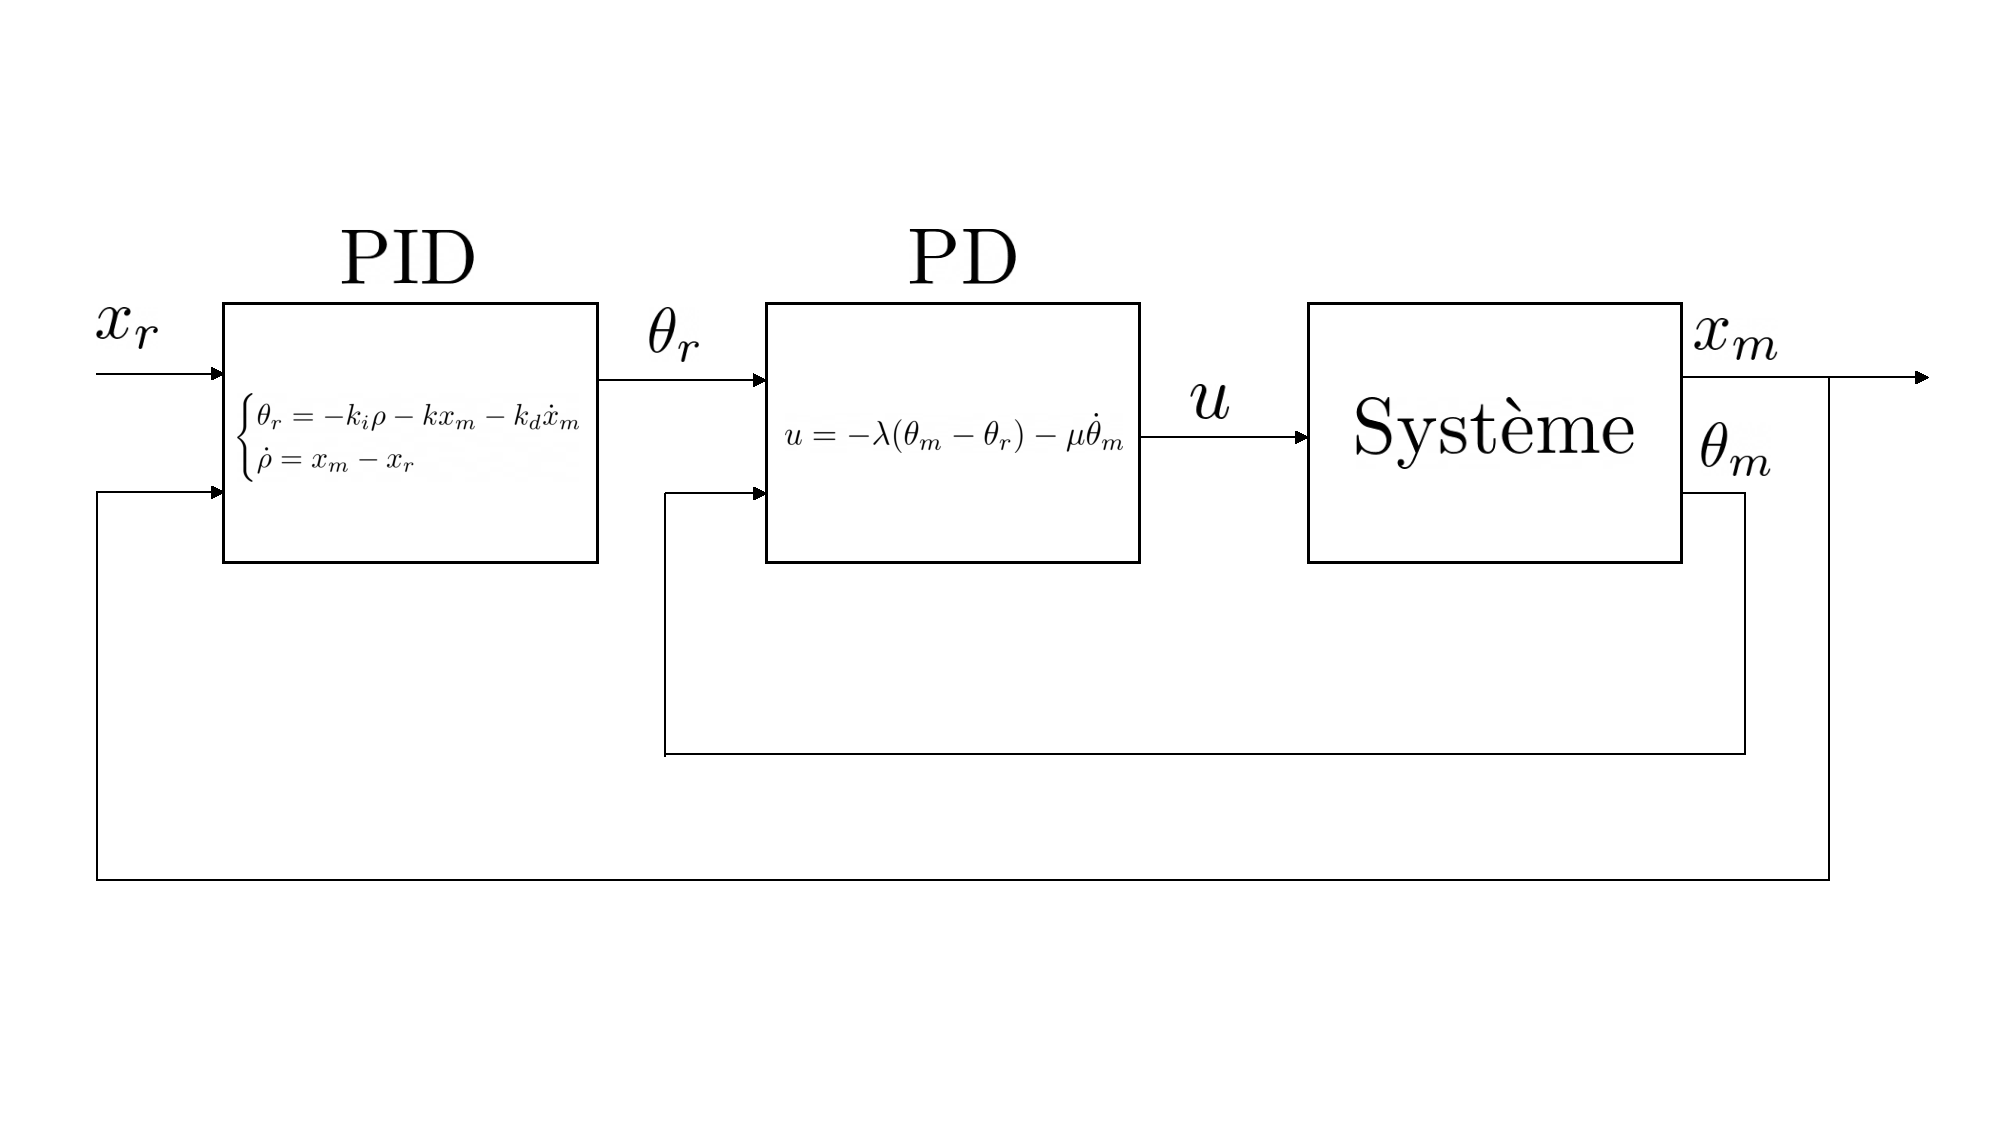
\includegraphics[width=\linewidth]{schemaPD+PID.pdf}
	\caption{Architecture du système bouclé}
\end{figure}

\subsection*{Paramétrage du système rapide}

\noindent En négligeant toujours les bruits de mesure, le système rapide vérifie :

\[
	\begin{cases}
		\dot \theta = q \\
		\dot q =
		\frac{gx \cos \theta - \lambda ( \theta + k_i \eta + k x + k_d v ) - \mu q + d - 2xqv}{\alpha + x^2}
	\end{cases}
\]

\noindent Cela donne le linéarisé, en notant $\gamma = \frac{1}{\alpha + \bar x^2} > 0$ :

\[
	\begin{bmatrix}
		\delta \dot \theta \\
		\delta \dot q
	\end{bmatrix}
	=\begin{bmatrix}
		0 & 1 \\
		- \gamma \lambda & - \gamma \mu
	\end{bmatrix}
	\begin{bmatrix}
		\delta \theta \\
		\delta q
	\end{bmatrix} +
	B_x \delta x +
	B_v \delta v +
	B_\eta \delta \eta +
	B_d \delta d
\]

\noindent Puis le polynôme caractéristique :

\[
	\begin{vmatrix}
		X & -1 \\
		\gamma \lambda & X + \gamma \mu
	\end{vmatrix}
	= X^2 + \gamma \mu X + \gamma \lambda
\]

\noindent D'après le critère de Routh, le système rapide est donc stable si $\lambda > 0$ et $\mu > 0$. On souhaite
imposer un temps de réponse de $0,1 s$. On se propose d'identifier le polynôme caractéristique précédent avec
$X^2 + 2 \xi \omega_0 X + \omega_0^2$ où $\omega_0 = \frac{2 \pi}{0,1} = 20 \pi$ et $\xi = \frac{\sqrt 2}{2}$.
Alors :

\begin{align}
	\lambda &= \frac{\omega_0^2}{\gamma} = \frac{(20 \pi)^2}{\gamma} > 0 \notag \\
	\mu &= 20 \sqrt 2	 \pi > 0 \notag
\end{align}

\noindent Le critère de Routh est bien vérifié par ce paramétrage du système rapide.

\subsection*{Paramétrage du système lent}

\noindent La branche d'équilibre est donnée par : ...

\[
	 \begin{cases}
	 	\dot x = v \\
		\dot v = g \sin \theta + x q^2 \\
		\dot \eta = x - x_r
	\end{cases}
\]



---------------------------------------------------------------------------------------------------


\noindent On obtient finalement le linéarisé puis le polynôme caractéristique suivants :

\[
	\delta \dot X' = \underbrace{
	\begin{bmatrix}
		0 & 1 & 0 \\
		- g k & - g k_d & - g k_i \\
		1 & 0 & 0
	\end{bmatrix}
	}_{\tilde A}
	\delta X'
	+
	\begin{bmatrix}
		0 \\
		0 \\
		- 1
	\end{bmatrix}
	\delta x_r
\]
\begin{align}
	\chi_{\tilde A} ( X) &=
	\begin{vmatrix}
		X & - 1 & 0 \\
		g k & X + g k_d & g k_i \\
		- 1 & 0 & X
	\end{vmatrix} \notag \\
	&= X^2 ( X + g k_d ) + g k X + g k_i \notag \\
	&= X^3 + g k_d X^2 + g k X + g k_i \notag
\end{align}

\subsection*{Paramétrage (attention au $\delta q$ pour l'instant)}

\noindent Le critère de Routh donne $k_d > 0$, $g k_i k > k_d$ et $g k_d k_i k > k_i^2$ pour que le système lent
soit stable.

\vspace{10px}

\noindent On va maintenant identifier le polynôme caractéristique $\chi_{\tilde A}$ avec ... qui donne de bonnes
performances tout en s'assurant que les inégalités issues du critère de Routh sont vérifiées.


\noindent Le système devient alors 
$\begin{bmatrix} 
	\dot x \\
	\dot v \\
	\dot \theta \\
	\dot q
\end{bmatrix} =
\begin{bmatrix} 
	v \\
	x q^2 + g \sin \theta \\
	q \\ 
	\frac{gx \cos \theta - \lambda ( \theta + k_i \eta + k x + k_d v ) + d - 2xqv}{\alpha + x^2}
\end{bmatrix}$.

\vspace{10px}

\noindent Le système étant rapide,
on considère $\lambda$ grand donc $\varepsilon = \frac{1}{\lambda}$ petit. La dernière équation devient alors,
en négligeant toujours les deux bruits de mesure $\nu_x$ et $\nu_\theta$ :

\begin{align}
	\varepsilon \dot q &= \frac{\varepsilon gx \cos \theta - ( \theta + k_i \eta + k x + k_d v ) +
	\varepsilon d - 2 \varepsilon xqv}{\alpha + x^2} \notag \\
	&= - \frac{\theta + k_i \eta + k x + k_d v}{\alpha + x^2} + O (\varepsilon) \notag \\
	&:= g (x, v, \theta, q, \eta, \varepsilon) \notag
\end{align}

\noindent Si on fait maintenant $\varepsilon = 0$, on obtient l'équation algébrique :

\[
	0 = - \frac{\theta + k_i \eta + k x + k_d v}{\alpha + x^2}
\]

\noindent D'où la simplification :  $\theta = - k_i \eta - k x - k_d v \ (\star)$. La branche d'équilibre est ue-stable car :

\[
	\partial_{\theta} g |_{\theta = - k_i \eta - k x - k_d v} = - \frac{1}{\alpha + x^2} < 0
\]

\subsection*{Conclusion sur la question 2}

\fbox{
	\begin{minipage}{0.96\textwidth}
		Conclusion
	\end{minipage}
}

\subsection*{Conclusion sur la question 3}

\fbox{
	\begin{minipage}{0.96\textwidth}
		On impose $\bar u = ...$ de sorte à avoir $\bar x = 0,4$ avec la condition initiale $x_{t=0} = 0$.
	\end{minipage}
}

\end{document}










